% !TEX program = xelatex
% Informe final del proyecto, versión 5 (definitiva; sin sección de reproducibilidad, solo regresión lineal). Compilar desde paper/: python3 gen_anexos.py; xelatex informe_v5.tex (tres pasadas).
\documentclass[10.5pt,a4paper,headings=small,abstract=false,bibliography=totoc,listof=totoc]{scrartcl}

% ---------- Tipografía: TeX Gyre Pagella (texto, tablas y fórmulas), Figtree (títulos y rótulos)
\usepackage{fontspec}
\usepackage{polyglossia}
\setmainlanguage{spanish}
\addto\captionsspanish{%
 \renewcommand{\tablename}{Tabla}\renewcommand{\figurename}{Figura}\renewcommand{\refname}{Referencias}%
 \renewcommand{\contentsname}{Índice}\renewcommand{\listtablename}{Índice de tablas}\renewcommand{\listfigurename}{Índice de figuras}}
\setmainfont{texgyrepagella}[Extension=.otf,UprightFont=*-regular,BoldFont=*-bold,ItalicFont=*-italic,BoldItalicFont=*-bolditalic,Numbers={Lining,Monospaced}]
\setsansfont{Figtree}[Path=/home/diego/.fonts/,Extension=.ttf,UprightFont=*-Regular,BoldFont=*-Bold,ItalicFont=*-ItalicRegular,BoldItalicFont=*-Italic,Numbers={Lining,Monospaced}]
\usepackage{unicode-math}
\setmathfont{texgyrepagella-math.otf}[Path=/usr/share/texmf-dist/fonts/opentype/public/tex-gyre-math/]
\usepackage{microtype}

% ---------- Color
\usepackage{xcolor}
\definecolor{acento}{HTML}{0E5E5C}
\definecolor{acentoclaro}{HTML}{EEF5F4}
\definecolor{tinta}{HTML}{22343A}
\definecolor{gris}{HTML}{5F6F74}
\definecolor{filete}{HTML}{B9CFCD}

% ---------- Página y ritmo
\usepackage[a4paper,left=2.7cm,right=2.7cm,top=2.7cm,bottom=2.7cm]{geometry}
\usepackage{setspace}
\setstretch{1.0}
\setlength{\parindent}{0pt}
\setlength{\parskip}{0.4em}
\raggedbottom
\setlength{\textfloatsep}{10pt plus 2pt minus 2pt}\setlength{\floatsep}{8pt plus 2pt minus 2pt}\setlength{\intextsep}{8pt plus 2pt minus 2pt}
\setlength{\emergencystretch}{3em}
\tolerance=1200
\renewcommand{\topfraction}{0.9}\renewcommand{\floatpagefraction}{0.82}\setcounter{totalnumber}{4}
\usepackage{fancyhdr}
\pagestyle{fancy}\fancyhf{}
\renewcommand{\headrulewidth}{0pt}
\fancyhead[L]{\color{gris}\footnotesize Estadías hospitalarias en FONASA, 2020}
\fancyhead[R]{\color{gris}\footnotesize\thepage}
\fancypagestyle{plain}{\fancyhf{}\fancyhead[R]{\color{gris}\footnotesize\thepage}\renewcommand{\headrulewidth}{0pt}}

% ---------- Títulos
\setkomafont{disposition}{\sffamily\bfseries\color{acento}}
\setkomafont{section}{\sffamily\bfseries\color{acento}\Large}
\setkomafont{subsection}{\sffamily\bfseries\color{acento}\large}
\setkomafont{subsubsection}{\sffamily\bfseries\color{tinta}\normalsize}
\RedeclareSectionCommand[beforeskip=1.7em plus .3em minus .2em,afterskip=0.5em]{section}
\RedeclareSectionCommand[beforeskip=1.1em plus .2em minus .1em,afterskip=0.35em]{subsection}
\setkomafont{captionlabel}{\bfseries\color{acento}\footnotesize}
\setkomafont{caption}{\footnotesize\color{tinta}}
\color{tinta}

% ---------- Paquetes
\usepackage{amsmath}
\usepackage{graphicx}
\usepackage{booktabs}
\usepackage{colortbl}
\usepackage{array}
\usepackage{tabularx}
\usepackage{longtable}
\usepackage{float}
\usepackage{caption}
\usepackage{tikz}
\usetikzlibrary{arrows.meta,positioning}
\usepackage{url}\urlstyle{same}
\usepackage[colorlinks=true,linkcolor=acento,citecolor=acento,urlcolor=acento]{hyperref}
\usepackage[authoryear,round]{natbib}
\setcitestyle{aysep={,}}
\setlength{\bibhang}{1.27cm}
\captionsetup{font=small,justification=raggedright,singlelinecheck=false,labelsep=period,skip=6pt}
\captionsetup[table]{position=above}
\captionsetup[figure]{position=above}
\renewcommand{\arraystretch}{1.14}
\arrayrulecolor{filete}
\setlength{\heavyrulewidth}{0.9pt}\setlength{\lightrulewidth}{0.4pt}

% ---------- Índice
\setcounter{tocdepth}{2}
\DeclareTOCStyleEntry[entryformat=\sffamily\bfseries\color{acento},pagenumberformat=\sffamily\bfseries\color{acento},beforeskip=0.6em]{tocline}{section}
\DeclareTOCStyleEntry[beforeskip=0.1em]{tocline}{subsection}

\newcommand{\fuente}{\par\vspace{0.3em}{\footnotesize\color{gris}Fuente: DEIS, MINSAL, egresos hospitalarios 2020; elaboración propia.\par}}
\newcommand{\fuentepropia}{\par\vspace{0.3em}{\footnotesize\color{gris}Fuente: elaboración propia.\par}}
\newcolumntype{Y}{>{\raggedright\arraybackslash}X}
\newcommand{\cie}{\mbox{CIE-10}}
\newcommand{\pct}{\,\%}
\newcommand{\filas}{\rowcolors{2}{white}{acentoclaro}}
\newcommand{\anexo}[1]{anexo~\ref{#1}}
\makeatletter\let\inputtab\@@input\makeatother

\title{Factores asociados a la duración de la estadía hospitalaria en beneficiarios FONASA, Chile 2020}
\author{Diego Muñoz y Franco Pastorini}
\date{10 de noviembre de 2026}

\begin{document}

% =====================================================================
% Portada
\begin{titlepage}
\pagenumbering{roman}
\thispagestyle{plain}
\raggedright
\vspace*{5.5cm}
{\sffamily\bfseries\color{acento}\fontsize{24}{29}\selectfont Factores asociados a la duración de la estadía hospitalaria en beneficiarios FONASA, Chile 2020\par}
\vspace{1.2em}
{\color{gris}\large Informe final del proyecto de investigación\par}
\vspace{0.3em}
{\color{gris}\large Universidad del Desarrollo\par}
\vspace{0.8em}
{\color{filete}\rule{\textwidth}{0.6pt}}\par
\vfill
{\sffamily\bfseries\large Diego Muñoz\par Franco Pastorini\par}
\vspace{1.4em}
{\small
\begin{tabular}{@{}l@{\hspace{1.2em}}l@{}}
\color{gris}Asignatura & Análisis de Datos e Inferencia Estadística \\
\color{gris}Profesor & Danilo Gómez Correa \\
\multicolumn{2}{@{}l@{}}{Certamen 2, 10 de noviembre de 2026} \\
\end{tabular}\par}
\vspace{1cm}
\end{titlepage}
\setcounter{page}{2}

% =====================================================================
% Resumen
{\sffamily\bfseries\color{acento}\Large Resumen}\par\vspace{0.6em}
\addcontentsline{toc}{section}{Resumen}
Estudiamos los 968.098 egresos FONASA de 2020 publicados por el DEIS. Las estadías de más de 15 días son el 9,4\pct{} de los egresos, porque el corte es el percentil 90 de la duración, pero usan el 47,1\pct{} de los días-cama. Evaluamos qué factores clínicos, demográficos y del sistema de salud se asocian con la duración de la estadía y qué tan grande es cada asociación. Usamos la base completa, así que las medidas de ajuste describen esta población. Una regresión lineal múltiple de $\ln$(días) explica el 19,8\pct{} de la variación ($R^2$ ajustado $=0{,}198$). Rechazamos la hipótesis nula general y las de cada grupo de factores. Al ordenar los factores por su tamaño de efecto ajustado, el capítulo \cie{} queda primero ($\eta^2$ parcial $=0{,}074$), seguido del tipo de establecimiento ($0{,}041$) y de la edad ($0{,}035$); la selección forward por BIC los incorpora en el mismo orden. Frente a los egresos de establecimientos fuera del SNSS, los del SNSS tienen una media geométrica de días 70,0\pct{} mayor. Sexo, cirugía, condición de egreso y región son significativos, pero su aporte es menor que un efecto pequeño. Como la base no trae gravedad ni identificadores de paciente y hospital, las asociaciones no son causales.

\vspace{0.4em}
{\small\color{gris}\textbf{Palabras clave:} estadía hospitalaria, FONASA, regresión lineal múltiple, tamaño del efecto, \cie.\par}

\clearpage
% =====================================================================
% Índices
\tableofcontents
\vspace{1.2em}
\listoftables
\vspace{1.2em}
\listoffigures

\clearpage
\pagenumbering{arabic}

% =====================================================================
\section{Introducción}

La gestión de camas depende de cuánto dura cada hospitalización, y esa duración es muy desigual. En los egresos FONASA de 2020 la mitad dura 3 días o menos, pero las estadías de más de 15 días ocupan casi la mitad de los días-cama. Saber qué se asocia a la duración ayuda a entender dónde se concentra el uso de camas.

La pregunta de investigación es:

\begin{quote}
\emph{¿Qué factores clínicos, demográficos y del sistema de salud se asocian con la duración de la estadía en los egresos FONASA de Chile en 2020?}
\end{quote}

Llamamos prolongada a una estadía de más de 15 días, el percentil 90 de la duración, así que por construcción cerca de uno de cada diez egresos queda como prolongado. Ese corte solo se usa para describir la concentración de días-cama y en las pruebas chi-cuadrado de a pares. La hipótesis general es:

\begin{itemize}\setlength\itemsep{0pt}
\item $H_0$: la duración de la estadía no se asocia con los factores clínicos, demográficos ni del sistema de salud.
\item $H_1$: al menos uno de esos factores se asocia con la duración de la estadía.
\end{itemize}

La separamos en una hipótesis por grupo de factores. En cada una, la nula dice que ningún factor del grupo se asocia con la duración una vez que los demás factores se mantienen constantes, y la alternativa dice que al menos uno sí se asocia.

\begin{itemize}\setlength\itemsep{0pt}
\item $H_{0a}$ y $H_{1a}$ (clínicos): capítulo del diagnóstico (\cie), cirugía y condición de egreso.
\item $H_{0b}$ y $H_{1b}$ (demográficos): edad y sexo. Esperamos más días a mayor edad.
\item $H_{0c}$ y $H_{1c}$ (sistema de salud): tipo de establecimiento y región.
\item $H_{0d}$ y $H_{1d}$ (sensibilidad): nacionalidad y etnia, que la selección de variables dejó fuera. La nula dice que no agregan asociación con la duración a los siete factores anteriores.
\end{itemize}

Cada hipótesis se contrasta con pruebas formales, que resume la tabla~\ref{tab:pruebasH}. Con casi un millón de egresos, un valor-$p$ bajo no basta para decir que un factor importa, así que también ordenamos los factores según su tamaño de efecto (sección~\ref{sec:ranking}).

% =====================================================================
\section{Revisión de literatura}

Los Grupos Relacionados por el Diagnóstico (GRD) agrupan a los pacientes según su diagnóstico y sus procedimientos, porque esas dos cosas explican buena parte de los recursos que consume una hospitalización y de lo que dura \citep{fetter1980}. \citet{freitas2012} analizaron 9 millones de hospitalizaciones en Portugal y encontraron que la edad y el tipo de hospital seguían asociados a las estadías extremas dentro de un mismo GRD. Por eso no nos quedamos solo con el diagnóstico: incluimos factores del paciente y del establecimiento.

\citet{gomez2023} modelaron la estadía media de un hospital de Medellín con regresión lineal múltiple, elegida por AIC y BIC y contrastada con la $F$ global, como hacemos aquí. Su determinante más fuerte fue la complejidad de los casos, con $R^2$ ajustado de 0,82. Ese valor usa promedios agregados y medidas de complejidad que el DEIS no trae, así que no se compara directo con el nuestro. Aun así, es posible que la gravedad explique buena parte de lo que un modelo por egreso deja fuera. Para revisar los supuestos del estimador de mínimos cuadrados ordinarios seguimos a \citet{rodriguez2017}.

Con bases de este tamaño casi cualquier diferencia sale significativa. \citet{lin2013} recomiendan reportar el tamaño del efecto junto con el valor-$p$, y nosotros lo interpretamos con los umbrales de \citet{cohen1988}. En las pruebas no paramétricas, el tamaño del efecto de dos grupos es la correlación biserial de rangos \citep{kerby2014}. \citet{raftery1995} plantea el mismo problema para la selección de modelos: con muestras grandes, elegir variables por su valor-$p$ deja variables que casi no aportan. Propone el criterio de información bayesiano (BIC; \citealt{schwarz1978}), que usamos para decidir qué variables entran a los modelos.

En Chile, \citet{olivares2020} estudió las estadías largas, pero solo en adultos mayores. No encontramos un trabajo que mire a la vez factores clínicos, demográficos y del sistema de salud en el total de egresos FONASA, ni uno sobre 2020, el primer año de la pandemia. Ese año no fue típico: con los mismos registros del DEIS, \citet{barahona2021} muestran que los egresos del país bajaron 19\pct{} frente a 2019, mientras se suspendían cirugías electivas y se reconvertían camas. Como la base abierta no trae peso GRD ni gravedad, la pregunta de fondo es cuánto de la duración se asocia con las variables que sí están disponibles.

% =====================================================================
\section{Metodología}

\subsection{Diseño del estudio}

Es un estudio observacional retrospectivo y analítico. Describe la distribución de la duración, contrasta las hipótesis con pruebas de asociación y estima asociaciones ajustadas con modelos de regresión. Todos los modelos se estiman con los 968.098 egresos y sus medidas de ajuste ($R^2$, BIC) describen esta población. Para los valores-$p$ y los intervalos tratamos los egresos de 2020 como una realización del proceso que generó las hospitalizaciones de ese año, de modo que miden la incertidumbre de las estimaciones bajo esas condiciones. La figura~\ref{fig:diagrama} resume el flujo.

\begin{figure}[!htb]
\centering
\caption{Diagrama metodológico.}
\label{fig:diagrama}
\begin{tikzpicture}[node distance=0.25cm, every node/.style={font=\fontsize{7.6}{9}\selectfont\sffamily},
 caja/.style={draw=acento, rounded corners=2pt, minimum width=2.25cm, minimum height=1.45cm, text width=2.05cm, align=center, fill=acentoclaro},
 flecha/.style={-{Stealth[length=1.8mm]}, thick, color=acento}]
\node[caja] (a) {\textbf{Problema}\\ duración de la estadía};
\node[caja, right=of a] (b) {\textbf{Datos}\\ DEIS 2020, 968.098 egresos};
\node[caja, right=of b] (c) {\textbf{Procesamiento}\\ filtros, variables, exploración};
\node[caja, right=of c] (d) {\textbf{Asociaciones}\\ pruebas de a pares, tamaño del efecto};
\node[caja, right=of d] (e) {\textbf{Modelamiento}\\ regresión lineal, sensibilidad};
\node[caja, right=of e] (f) {\textbf{Evaluación}\\ supuestos, $F$, BIC, $\eta^2$, ranking};
\foreach \i/\j in {a/b,b/c,c/d,d/e,e/f} \draw[flecha] (\i)--(\j);
\end{tikzpicture}
{\footnotesize\color{gris}Fuente: elaboración propia.\par}
\end{figure}

\subsection{Datos}

La fuente son los egresos hospitalarios 2020 del DEIS-MINSAL (datos abiertos). Usamos solo egresos FONASA (\texttt{PREVISION = 1}) con estadías de hasta 365 días, como en el Avance 1. Excluimos 397 egresos (0,04\pct{}) de más de un año por esa regla de depuración. El máximo es de 16.598 días, unos 45 años, y la duración por sí sola no demuestra que todos sean errores de registro. Quedan 968.098 egresos, dentro del rango pedido de 700.000 a 1.000.000. La unidad de análisis es el egreso, no el paciente.

\subsection{Variables}

La base trae 18 columnas. Revisamos cada una con tres condiciones: que su significado esté en el diccionario del DEIS o se pueda verificar con los datos, que varíe entre egresos y que no repita otra columna. Quedaron nueve variables candidatas y la respuesta (tabla~\ref{tab:vars}). \texttt{DIAG2} se descarta porque está vacía en el 90,2\pct{} de los egresos. \texttt{COMUNA\_RESIDENCIA} repite la región con 344 categorías. \texttt{PROCED} no está en el diccionario y no pudimos verificar qué registra. \texttt{INTERV\_Q} tampoco está, pero su codificación calza con cirugía: por ejemplo, vale 1 en el 97\pct{} de las cesáreas.

\begin{table}[!htb]
\centering\footnotesize\filas
\caption{Variables del estudio.}
\label{tab:vars}
\begin{tabularx}{\textwidth}{>{\raggedright\arraybackslash}p{2.9cm} >{\raggedright\arraybackslash}p{3.7cm} >{\raggedright\arraybackslash}p{2.6cm} Y}
\toprule
Variable & Columna & Tipo & Justificación \\
\midrule
Días de estada & \texttt{DIAS\_ESTADA} & Numérica & Respuesta de la regresión lineal (en $\ln$) \\
Estadía prolongada & días $>15$ & Categórica (Sí/No) & Solo descriptiva y en el chi-cuadrado de a pares \\
Capítulo \cie & \texttt{DIAG1} & Categórica (21) & Aproxima la gravedad, porque no hay peso GRD \\
Cirugía & \texttt{INTERV\_Q} & Categórica (Sí/No) & Distingue casos quirúrgicos de médicos \\
Condición de egreso & \texttt{CONDICION\_EGRESO} & Categórica (vivo/fallecido) & Los fallecidos suelen ser casos graves \\
Edad & \texttt{GRUPO\_EDAD} & Numérica (punto medio) & Más edad, más días \citep{freitas2012} \\
Sexo & \texttt{SEXO} & Categórica & Variable demográfica básica \\
Nacionalidad & \texttt{GLOSA\_PAIS\_ORIGEN} & Categórica (2) & Revisar si el origen cambia la duración \\
Etnia & \texttt{ETNIA} & Categórica (Sí/No) & Revisar pertenencia a pueblo originario \\
Establecimiento & \texttt{PERTENENCIA\_...} & Categórica (SNSS/No SNSS) & Tipo de hospital \citep{freitas2012} \\
Región & \texttt{REGION\_RESIDENCIA} & Categórica (16) & Acceso y oferta de camas \\
\bottomrule
\end{tabularx}
\fuentepropia
\end{table}

La condición de egreso se conoce recién al alta, así que los modelos no sirven como herramienta de decisión al ingreso.

\subsection{Pruebas de hipótesis}\label{sec:pruebas}

Usamos $\alpha=0{,}05$ en todas las pruebas. La tabla~\ref{tab:pruebasH} muestra la hipótesis nula y la alternativa de cada prueba. Las primeras cinco filas son las pruebas de a pares del Avance 1, que miran cada factor por separado. Las demás contrastan las hipótesis de la introducción dentro de los modelos, con los otros factores constantes: $H_{0a}$, $H_{0b}$ y $H_{0c}$ se rechazan si la prueba $F$ parcial (o la $t$, en la edad) de alguno de sus factores en M3 tiene $p<0{,}05$. $H_{0d}$ se contrasta con la $F$ parcial de nacionalidad y etnia agregadas a M3. Con este tamaño de muestra rechazar es casi seguro, así que la conclusión también usa el criterio de relevancia de la sección~\ref{sec:lineal}.

\begin{table}[!htb]
\centering\footnotesize\filas
\caption{Hipótesis de cada prueba. $\beta$ son coeficientes del modelo lineal.}
\label{tab:pruebasH}
\setlength{\tabcolsep}{4pt}\begin{tabularx}{\textwidth}{>{\raggedright\arraybackslash}p{2.75cm} >{\raggedright\arraybackslash}p{3.0cm} Y >{\raggedright\arraybackslash}p{2.3cm} >{\raggedright\arraybackslash}p{1.75cm}}
\toprule
Prueba & Se aplica a & $H_0$ & $H_1$ & Estadístico \\
\midrule
Shapiro--Wilk, Lilliefors, A--D & Días y edad & La variable sigue una distribución normal & No la sigue & $W$, $D$, $A^2$ \\
Spearman & Edad y días & $\rho_s=0$ & $\rho_s\neq0$ & $\rho_s$ \\
Mann--Whitney U & Días según un factor de dos grupos & Ambos grupos tienen la misma distribución de días & Un grupo tiende a más días & $U$; $r$ \\
Kruskal--Wallis + Holm & Días según capítulo o región & Todos los grupos tienen la misma distribución & Al menos un grupo difiere & $H$; $\varepsilon^2$ \\
Chi-cuadrado de independencia & Factor y estadía prolongada (bivariado) & Son independientes & No son independientes & $\chi^2$; $V$ \\
$F$ global (ANOVA) & Modelo lineal M3 & Todos los $\beta_j=0$ salvo el intercepto & Algún $\beta_j\neq0$ & $F$ \\
$F$ parcial & Cada bloque (M1 a M3) y cada factor retirado de M3 & Los coeficientes del factor valen 0 & Alguno es distinto de 0 & $F$; $\eta^2$ parcial \\
$t$ (EE clásico, HC3) & Cada coeficiente de M3 & $\beta_j=0$ & $\beta_j\neq0$ & $t$ \\
\bottomrule
\end{tabularx}
\fuentepropia
\end{table}

Verificamos la normalidad de las variables numéricas con Shapiro--Wilk \citep{shapiro1965} (en una muestra de 5.000 egresos, porque con más datos su valor-$p$ deja de ser exacto), Kolmogorov--Smirnov con corrección de Lilliefors \citep{lilliefors1967} y Anderson--Darling. Como la normalidad se rechaza, usamos pruebas no paramétricas para los pares: Spearman en vez de Pearson, Mann--Whitney en vez de $t$ de Student (por eso no aplica Levene) y Kruskal--Wallis en vez de ANOVA de un factor, con comparaciones post hoc de Mann--Whitney ajustadas por Holm \citep{holm1979} en vez de Tukey HSD. Hacemos 20 pruebas de a pares. Con la corrección de Bonferroni el nivel sería $0{,}05/20=0{,}0025$ y ninguna decisión cambia: las 18 pruebas de asociación tienen $p<0{,}0002$, y la normalidad se rechaza igual porque Shapiro--Wilk y Lilliefors tienen $p<0{,}001$ (Anderson--Darling solo informa $p\le0{,}01$). El \anexo{anx:pares} reporta para cada una sus hipótesis, el estadístico, el valor-$p$, la decisión y el tamaño del efecto.

Los umbrales de \citet{cohen1988} para efecto pequeño, mediano y grande son 0,1, 0,3 y 0,5 en $\rho$, $r$ y $V$ de Cramér, y 0,01, 0,06 y 0,14 en $\varepsilon^2$ y $\eta^2$.

\subsection{Selección de variables}

En el Avance 1 ajustamos un modelo lineal de $\ln$(días) con las nueve candidatas y eliminamos hacia atrás según el $\mathrm{BIC}=n\,[\ln(2\pi)+1+\ln(\mathrm{SCR}/n)]+k\ln n$, donde SCR es la suma de cuadrados de los residuos y $k$ el número de coeficientes. Cada coeficiente cuesta $\ln(968.098)\approx 13{,}8$. Para una variable de un coeficiente, eso equivale a exigir un $F$ parcial mayor que 13,8 en vez del 3,84 que pide $p<0{,}05$ \citep{raftery1995}. Quedaron siete variables: capítulo, cirugía, condición de egreso, edad, sexo, establecimiento y región. Nacionalidad y etnia salieron, y revisamos su incorporación como sensibilidad ($H_{0d}$).

\subsection{Regresión lineal múltiple}\label{sec:lineal}

Estimamos por mínimos cuadrados ordinarios el modelo M3, con los siete factores a la vez para describir la asociación de cada uno con los demás constantes:
\begin{multline*}
\ln(\text{días}_i)=\beta_0+\sum_c\gamma_c\,\text{capítulo}_{ic}+\beta_1\,\text{cirugía}_i+\beta_2\,\text{fallecido}_i+\beta_3\,\text{edad}_{c,i}\\
+\beta_4\,\text{edad}_{c,i}^2+\beta_5\,\text{hombre}_i+\beta_6\,\text{SNSS}_i+\sum_r\delta_r\,\text{región}_{ir}+\varepsilon_i .
\end{multline*}
La referencia de capítulo es K00--K93 (digestivo): tiene hombres y mujeres y una mediana de 2 días, así que los demás capítulos se leen como diferencias respecto de un egreso corto y habitual. No usamos O00--O99 porque solo tiene mujeres. La referencia de región es la Región Metropolitana, el sexo de referencia es mujer y la edad está centrada en su media (45,01 años).

Como el modelo describe la media condicional de $\ln$(días), su exponencial es una media geométrica condicional. Por eso interpretamos $100\,(e^{\beta}-1)\pct{}$ como el cambio porcentual en la media geométrica de los días.

Para ver cuánto aporta cada bloque ajustamos cuatro modelos anidados: M0 (solo intercepto), M1 (bloque clínico), M2 (M1 más edad, edad$^2$ y sexo) y M3 (M2 más establecimiento y región). Comparamos BIC, $F$ parcial y $\eta^2$ parcial. El $\eta^2$ parcial de un bloque o factor es la parte de la variación que quedaba sin explicar y que su inclusión explica:
\[
\eta^2_{\text{parcial}}=\frac{R^2_{\text{con}}-R^2_{\text{sin}}}{1-R^2_{\text{sin}}}.
\]
Como el aporte secuencial depende del orden en que entran los bloques, también retiramos cada factor de M3 y medimos cuánto baja el $R^2$. Un factor es relevante si, además de significativo, su $\eta^2$ parcial es de al menos 0,01. Este umbral es un criterio práctico y no una prueba: con casi un millón de egresos, el valor-$p$ no distingue entre efectos grandes y pequeños.

\subsection{Criterio para el ranking}

Para ordenar los factores usamos su tamaño de efecto ajustado, porque todos tienen $p<0{,}001$ y el valor-$p$ no los separa. El orden es el $\eta^2$ parcial de cada factor al retirarlo de M3. Lo contrastamos con el orden en que entra en una selección forward por BIC. El $\eta^2$ parcial no se corrige por grados de libertad, así que un factor con muchas categorías, como el capítulo (20 gl), puede acumular más que uno binario. De a pares solo comparamos la categoría de Cohen, porque $\rho$, $r$, $\varepsilon^2$ y $V$ no están en la misma escala.

\subsection{Métricas de evaluación}

Como el objetivo es describir asociaciones, evaluamos los modelos con medidas de ajuste e inferencia sobre la base completa: $R^2$ ajustado, BIC y AIC, pruebas $F$ y $t$, $\eta^2$ parcial e intervalos de confianza, con errores estándar HC3 como contraste de los clásicos.

\subsection{Supuestos y sensibilidad}

Revisamos la forma funcional, el rango de la matriz de diseño, la multicolinealidad con el VIF, la heterocedasticidad y la distribución de los residuos. Como la varianza de los residuos no es constante, reportamos además errores estándar robustos HC3 \citep{long2000} para los coeficientes de M3. La exogeneidad, $E(\varepsilon\mid X)=0$, es un supuesto, y la independencia no se puede verificar con esta base porque no identifica pacientes ni hospitales. Como análisis de sensibilidad comparamos M3 con tres alternativas: M4 cambia edad y edad$^2$ por los 11 tramos de edad; M5 agrega la interacción capítulo $\times$ establecimiento; M6 agrega tramo de edad $\times$ establecimiento. También agregamos nacionalidad y etnia a M3 y repetimos la selección con un procedimiento forward por BIC.

% =====================================================================
\section{Resultados}

\subsection{Descripción y depuración}

Los días de estada tienen media 6,70 y mediana 3 (Q1 $=2$, Q3 $=7$). La desviación estándar (12,79) casi duplica la media y la asimetría es 9,04: la mayoría dura pocos días y unos pocos duran muchísimo (tabla~\ref{tab:desc} y figura~\ref{fig:dist}). En $\ln$(días) la asimetría baja a 0,68 y la media queda cerca de la mediana, por eso modelamos el logaritmo.

\begin{table}[!htb]
\centering\small\filas
\caption{Estadísticos descriptivos ($n=968.098$).}
\label{tab:desc}
\begin{tabular}{lrrrrr}
\toprule
Variable & Media & Mediana & Desv. est. & Asimetría & RIC \\
\midrule
Días de estada & 6,70 & 3,00 & 12,79 & 9,04 & 5,00 \\
$\ln$(días) & 1,25 & 1,10 & 1,04 & 0,68 & 1,25 \\
Edad (años) & 45,01 & 44,50 & 24,29 & 0,01 & 40,00 \\
\bottomrule
\end{tabular}
\fuente
\end{table}

\begin{figure}[!htb]
\centering
\caption{Distribución de los días de estada (izquierda, recortada a 60 días), de $\ln$(días) (centro) y curva de concentración de los días-cama (derecha). Los egresos de más de 15 días son el 9,4\pct{} y usan el 47,1\pct{} de los días-cama.}
\label{fig:dist}
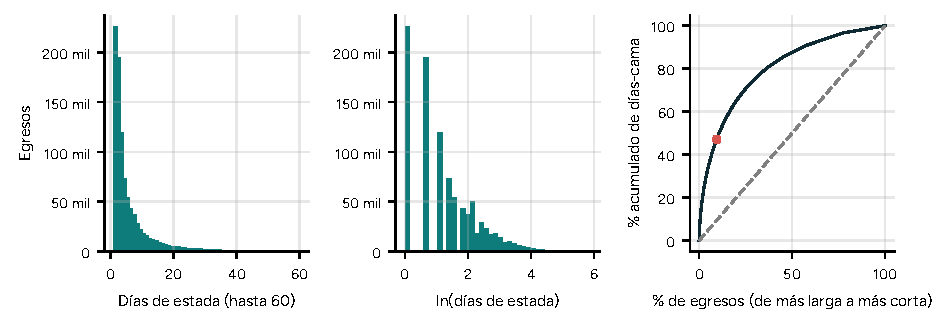
\includegraphics[width=0.86\textwidth]{figs/avance2_distribucion.pdf}
\fuente
\end{figure}

El 81,8\pct{} de los egresos son de establecimientos del SNSS y el 60,0\pct{} son de mujeres. Los capítulos más frecuentes son embarazo, parto y puerperio (O00--O99, 20,4\pct{}), digestivo (K00--K93, 13,8\pct{}) y traumatismos (S00--T98, 9,8\pct{}). La respuesta y las siete variables explicativas no tienen valores nulos, así que no imputamos ni eliminamos egresos.

Con el criterio de Tukey, 99.978 egresos (10,33\pct{}) superan los 14,5 días; no los eliminamos porque son justamente las estadías que estudiamos. Con los 397 egresos de más de 365 días, la media subiría de 6,70 a 7,29 y la desviación estándar de 12,79 a 59,74, sin cambiar la mediana (3) ni el MAD (2).

\subsection{Normalidad y asociaciones de a pares}

Las tres pruebas rechazan la normalidad de los días y de la edad (Shapiro--Wilk y Lilliefors con $p<0{,}001$; Anderson--Darling con $p\le0{,}01$, porque \texttt{scipy} no informa valores menores). Por eso usamos pruebas no paramétricas.

La edad se relaciona con los días con $\rho=0{,}25$ ($p<0{,}001$): a mayor edad la estadía tiende a ser más larga, con un efecto pequeño. La mediana sube de 2 días en adultos jóvenes a 6 días desde los 80 años, con la excepción de los menores de un año (mediana de 4 días). Con Mann--Whitney y Kruskal--Wallis todos los factores rechazan $H_0$ ($p<0{,}001$), pero con efectos distintos. El establecimiento ($r=-0{,}37$, mediano) y el capítulo ($\varepsilon^2=0{,}12$, mediano) son los mayores; condición de egreso, cirugía y sexo tienen efectos pequeños; nacionalidad, etnia y región son despreciables (figura~\ref{fig:biv}). Con Holm, 202 de los 210 pares de capítulos y 104 de los 120 pares de regiones difieren. En el chi-cuadrado sobre la estadía prolongada, todas las frecuencias esperadas superan 5 (la menor es 175) y la asociación más fuerte es la del capítulo ($V=0{,}25$, de 0,9\pct{} de prolongadas en embarazo y parto a 35,6\pct{} en trastornos mentales). La edad tiene forma de U: 15,4\pct{} de prolongadas en menores de un año, 3,5\pct{} entre 20 y 29 años y 15,4\pct{} entre 70 y 79. La tabla~\ref{tab:resumen} resume las pruebas. El \anexo{anx:pares} trae el detalle de cada una, los gráficos Q-Q, los boxplots de los demás factores y las tablas de contingencia con sus barras apiladas.

\begin{table}[!htb]
\centering\footnotesize\filas
\caption{Resumen de las pruebas de a pares ($\alpha=0{,}05$). El estadístico y los grados de libertad de cada prueba están en la tabla~\ref{tab:anx-pares}.}
\label{tab:resumen}
\setlength{\tabcolsep}{4pt}\begin{tabularx}{\textwidth}{>{\raggedright\arraybackslash}p{2.6cm} >{\raggedright\arraybackslash}p{1.7cm} >{\raggedright\arraybackslash}p{2.6cm} >{\raggedright\arraybackslash}p{1.25cm} >{\raggedright\arraybackslash}p{1.55cm} Y}
\toprule
Variable 1 & Variable 2 & Prueba & Valor-$p$ & Decisión & Conclusión \\
\midrule
Días y edad & Normalidad & Shapiro--Wilk, Lilliefors, A--D & ${\le}0{,}01$ & Rechaza $H_0$ & No son normales \\
Edad & Días & Spearman & $<0{,}001$ & Rechaza $H_0$ & $\rho=0{,}25$ (pequeño) \\
Establecimiento & Días & Mann--Whitney U & $<0{,}001$ & Rechaza $H_0$ & SNSS más largas ($r=-0{,}37$, mediano) \\
Capítulo \cie & Días & Kruskal--Wallis + Holm & $<0{,}001$ & Rechaza $H_0$ & Mediana de 1 a 9 días ($\varepsilon^2=0{,}12$, mediano) \\
Condición de egreso & Días & Mann--Whitney U & $<0{,}001$ & Rechaza $H_0$ & Fallecidos más largas ($r=-0{,}29$, pequeño) \\
Cirugía & Días & Mann--Whitney U & $<0{,}001$ & Rechaza $H_0$ & Sin cirugía más largas ($r=0{,}22$, pequeño) \\
Sexo & Días & Mann--Whitney U & $<0{,}001$ & Rechaza $H_0$ & Hombres más largas ($r=0{,}14$, pequeño) \\
Nacionalidad, etnia & Días & Mann--Whitney U & $<0{,}001$ & Rechaza $H_0$ & Despreciable ($r=0{,}06$ y $-0{,}02$) \\
Región & Días & Kruskal--Wallis + Holm & $<0{,}001$ & Rechaza $H_0$ & Despreciable ($\varepsilon^2=0{,}002$) \\
Capítulo \cie & Prolongada & Chi-cuadrado & $<0{,}001$ & Rechaza $H_0$ & $V=0{,}25$ (pequeño) \\
Tramo de edad & Prolongada & Chi-cuadrado & $<0{,}001$ & Rechaza $H_0$ & Forma de U ($V=0{,}16$, pequeño) \\
Condición de egreso & Prolongada & Chi-cuadrado & $<0{,}001$ & Rechaza $H_0$ & 25,3\pct{} frente a 8,8\pct{} ($V=0{,}11$, pequeño) \\
Sexo & Prolongada & Chi-cuadrado & $<0{,}001$ & Rechaza $H_0$ & 13,1\pct{} frente a 6,9\pct{} ($V=0{,}10$, pequeño) \\
Establecimiento & Prolongada & Chi-cuadrado & $<0{,}001$ & Rechaza $H_0$ & 10,6\pct{} frente a 4,2\pct{} ($V=0{,}08$, despreciable) \\
Cirugía, región, nacionalidad, etnia & Prolongada & Chi-cuadrado & $\le0{,}0002$ & Rechaza $H_0$ & Despreciable ($V<0{,}06$) \\
\bottomrule
\end{tabularx}
\fuente
\end{table}

\begin{figure}[!htb]
\centering
\caption{Distribución de $\ln$(días) por capítulo \cie{} (ordenado por mediana), por tipo de establecimiento y por sexo. Sin puntos atípicos, para ver las cajas. La mediana de días va de 1 (H00--H59) a 9 (U00--U99).}
\label{fig:biv}
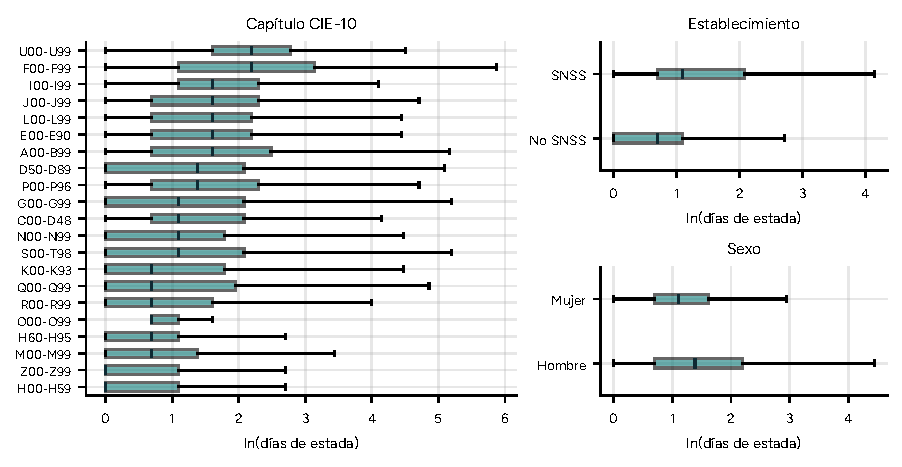
\includegraphics[width=0.8\textwidth]{figs/avance2_bivariado.pdf}
\fuente
\end{figure}

Con este tamaño de muestra, hasta una $V$ de 0,004 sale significativa. Entre las variables explicativas categóricas, la asociación más alta es la de capítulo con cirugía y con sexo ($V=0{,}43$ en ambos; en el sexo por el 100\pct{} de mujeres en O00--O99), seguida de cirugía con establecimiento ($0{,}28$) y de capítulo con condición de egreso ($0{,}26$). Son asociaciones de pequeñas a medianas, sin llegar a redundancia (figura~\ref{fig:cramer} del \anexo{anx:pares}).


\subsection{Modelos anidados}

La tabla~\ref{tab:anidados} muestra cuánto cambia el ajuste al incorporar cada bloque. El bloque clínico aporta más: el $R^2$ ajustado pasa de 0 a 0,132 y el BIC baja 137.235. Edad y sexo llevan el $R^2$ ajustado a 0,162, y establecimiento y región a 0,198. Todos los $F$ parciales tienen $p<0{,}001$ y el BIC baja en cada paso. M3 deja sin explicar cerca del 80,2\pct{} de la variación de $\ln$(días).

\begin{table}[!htb]
\centering\small\filas
\caption{Modelos anidados M0 a M3 en la base completa. $k$ es el número de coeficientes.}
\label{tab:anidados}
\begin{tabular}{lrrrrrrr}
\toprule
Modelo & $k$ & $R^2$ aj. & BIC & $\Delta$BIC & $F$ parcial & gl & $\eta^2$ parcial \\
\midrule
M0 & 1 & 0,000 & 2.814.166 & --- & --- & --- & --- \\
M1 & 23 & 0,132 & 2.676.930 & $-137.235$ & 6.717 & 22 & 0,132 \\
M2 & 26 & 0,162 & 2.643.664 & $-33.266$ & 11.295 & 3 & 0,034 \\
M3 & 42 & 0,198 & 2.601.099 & $-42.565$ & 2.734 & 16 & 0,043 \\
\bottomrule
\end{tabular}
\fuente
\end{table}


\subsection{Coeficientes de M3}

La tabla ANOVA del modelo completo da $F=5.830$ con 41 y 968.056 grados de libertad ($p<0{,}001$): la suma de cuadrados de la regresión es 205.399 sobre un total de 1.037.266. La tabla~\ref{tab:coef} muestra los coeficientes principales con su cambio porcentual en la media geométrica de los días, y el \anexo{anx:coef} trae los 42. Para el paciente de referencia (mujer, capítulo K00--K93, fuera del SNSS, sin cirugía, vivo, Región Metropolitana y edad media), la media geométrica es de 1,82 días.

\begin{table}[!htb]
\centering\small\filas
\caption{Coeficientes principales de M3 con error estándar clásico (EE) y robusto a heterocedasticidad (HC3). $\%\Delta=100\,(e^{\beta}-1)$, con intervalo de confianza del 95\pct{} clásico. En la fila de la edad, los errores estándar se muestran con seis decimales.}
\label{tab:coef}
\setlength{\tabcolsep}{4pt}
\begin{tabular}{lrrrr}
\toprule
Factor & $\hat\beta$ (EE) & EE HC3 & $\%\Delta$ & IC 95\pct \\
\midrule
Capítulo F00--F99 (mentales) & 1,147 (0,007) & 0,010 & $+214{,}8$ & 210,4 a 219,3 \\
Capítulo U00--U99 (uso especial) & 0,880 (0,005) & 0,006 & $+141{,}2$ & 138,6 a 143,8 \\
Capítulo P00--P96 (perinatal) & 0,805 (0,007) & 0,009 & $+123{,}8$ & 120,5 a 127,1 \\
Capítulo A00--B99 (infecciosas) & 0,643 (0,007) & 0,009 & $+90{,}3$ & 87,5 a 93,0 \\
Capítulo H00--H59 (ojo) & $-0{,}385$ (0,014) & 0,012 & $-31{,}9$ & $-33{,}7$ a $-30{,}1$ \\
Capítulo Z00--Z99 (factores de contacto) & $-0{,}356$ (0,007) & 0,007 & $-29{,}9$ & $-30{,}9$ a $-28{,}9$ \\
Cirugía & $-0{,}028$ (0,002) & 0,002 & $-2{,}8$ & $-3{,}2$ a $-2{,}3$ \\
Condición de egreso: fallecido & 0,061 (0,005) & 0,007 & $+6{,}3$ & 5,2 a 7,3 \\
Sexo: hombre & 0,107 (0,002) & 0,002 & $+11{,}3$ & 10,9 a 11,8 \\
Establecimiento: SNSS & 0,530 (0,003) & 0,002 & $+70{,}0$ & 69,1 a 70,8 \\
Edad (por año) & 0,009 (0,000048) & 0,000050 & $+0{,}89$ & 0,88 a 0,90 \\
\bottomrule
\end{tabular}
\fuente
\end{table}

Frente al digestivo, los trastornos mentales son el capítulo con mayor aumento y las enfermedades del ojo el de mayor disminución. Los hombres tienen más días que las mujeres con el mismo diagnóstico, edad y establecimiento. Entre regiones, Aisén tiene $-29{,}8\pct{}$ frente a la Región Metropolitana; sin ella el mínimo es $-15{,}8\pct{}$ y el máximo $+0{,}3\pct{}$. Las pruebas $F$ de tipo II rechazan la nulidad de cada factor (capítulo $F=3.867$ con 20 gl; región $F=310$ con 15 gl; establecimiento $F=41.287$). La figura~\ref{fig:forest} del \anexo{anx:coef} muestra el cambio porcentual de cada coeficiente con su intervalo.

La edad se estima con un término lineal y uno cuadrático. A los 74,5 años la media geométrica es 31,1\pct{} mayor que a la edad media. El modelo sigue la subida desde los 20 años y se aparta en los tramos extremos: en menores de un año ajusta 1,33 donde se observa 1,47 (figura~\ref{fig:edad} del \anexo{anx:supuestos}).

\subsection{Ajuste y supuestos}

Al comparar la media geométrica ajustada con la observada por decil de valor ajustado, las diferencias van en ambas direcciones: el decil 10 ajusta 8,05 días frente a 7,40 observados, y el decil 7 ajusta 4,18 frente a 4,56.

La matriz de diseño tiene rango completo (42 columnas) y el VIF máximo es 2,36, sin multicolinealidad problemática. La media de los residuos es 0 por construcción, lo que no prueba la exogeneidad. La varianza no es constante: la desviación estándar de los residuos pasa de 0,713 en el primer cuartil del valor ajustado a 1,061 en el cuarto. Los residuos tienen asimetría de 0,492 y curtosis en exceso de 0,542, y el gráfico Q-Q se aparta de la recta en las colas. Los gráficos de residuos y las tablas por decil y por tramo de edad están en el \anexo{anx:supuestos}. Por eso la tabla~\ref{tab:coef} incluye también los errores robustos HC3, que son entre 0,80 y 1,36 veces los clásicos. Ningún coeficiente deja de ser significativo, y el intervalo que más cambia (F00--F99) pasa de 210,4 a 219,3 a 208,8 a 220,9.

\subsection{Sensibilidad a la especificación}\label{sec:sens}

Los 11 tramos de edad (M4) suben el $R^2$ ajustado de 0,198 a 0,202, y la interacción capítulo $\times$ establecimiento (M5) lo lleva a 0,214 con $\eta^2$ parcial de 0,015. Es la única alternativa que pasa el umbral de 0,01: la diferencia del SNSS cambia según el diagnóstico, así que el +70,0\pct{} de M3, que mantenemos por ser más simple de leer, es un promedio sobre los capítulos. La interacción con la edad (M6) aporta 0,0008. El BIC más bajo es el de M6, pero su aporte es mínimo (\anexo{anx:sens}).

Nacionalidad y etnia rechazan $H_{0d}$ ($F=7{,}49$; $p=0{,}0006$), pero el $R^2$ ajustado no cambia (0,19799 frente a 0,19800), el BIC sube 12,6 y el $\eta^2$ parcial es 0,00002. La asociación existe, pero es tan pequeña que no justifica incluirlas.

\subsection{Ranking de variables}\label{sec:ranking}

La tabla~\ref{tab:ranking} ordena los factores por su $\eta^2$ parcial en M3. Tres factores pasan el umbral de 0,01: capítulo, establecimiento y edad. Los otros cuatro tienen $p<0{,}001$, pero su aporte ajustado es menor que un efecto pequeño. La selección forward por BIC agrega los factores en el mismo orden y termina en M3 sin descartar ninguno (\anexo{anx:sens}). Es una comprobación de coherencia, no independiente, porque usa los mismos datos. Con capítulo, establecimiento y edad, el $R^2$ ajustado ya llega a 0,192 de los 0,198 del modelo completo.

\begin{table}[!htb]
\centering\footnotesize\filas
\caption{Ranking de los factores según su tamaño de efecto ajustado: $\eta^2$ parcial al retirar el factor de M3. Todas las pruebas $F$ tienen $p<0{,}001$.}
\label{tab:ranking}
\setlength{\tabcolsep}{5pt}
\begin{tabular}{clrlcl}
\toprule
Pos. & Factor & $\eta^2$ parcial & Efecto & Paso forward & De a pares (días) \\
\midrule
1 & Capítulo \cie & 0,0740 & mediano & 1 & mediano \\
2 & Establecimiento & 0,0409 & pequeño & 2 & mediano \\
3 & Edad & 0,0347 & pequeño & 3 & pequeño \\
4 & Región & 0,0048 & menor que pequeño & 4 & despreciable \\
5 & Sexo & 0,0026 & menor que pequeño & 5 & pequeño \\
6 & Cirugía & 0,0002 & menor que pequeño & 6 & pequeño \\
7 & Condición de egreso & 0,0001 & menor que pequeño & 7 & pequeño \\
--- & Nacionalidad y etnia & 0,00002 & excluidas por BIC & --- & despreciable \\
\bottomrule
\end{tabular}
\fuente
\end{table}

De a pares el establecimiento ya tenía un efecto mediano sobre los días y la región era despreciable, lo que calza con su lugar en el ranking ajustado. La condición de egreso y la cirugía, en cambio, bajan al final del ranking: con el capítulo en el modelo, su aporte casi desaparece.

% =====================================================================
\section{Discusión}

\subsection{Respuesta a la pregunta y contraste de las hipótesis}

La $F$ global de M3 ($F=5.830$; $p<0{,}001$) rechaza la $H_0$ general, y la tabla~\ref{tab:hip} contrasta las hipótesis por grupo.

\begin{table}[!htb]
\centering\footnotesize\filas
\caption{Contraste de las hipótesis por grupo de factores ($\alpha=0{,}05$). $F$ de tipo II (o $t$, en la edad) en M3; todas con $p<0{,}001$ salvo donde se indica.}
\label{tab:hip}
\begin{tabularx}{\textwidth}{>{\raggedright\arraybackslash}p{2.2cm} Y >{\raggedright\arraybackslash}p{1.6cm} Y}
\toprule
Hipótesis & Prueba en M3 & Decisión & Relevancia ($\eta^2\ge0{,}01$) \\
\midrule
$H_{0a}$ clínicos & Capítulo $F=3.867$; cirugía $F=157$; fallecido $F=139$ & Rechaza $H_{0a}$ & Capítulo sí (0,074). Cirugía y fallecido no (0,0002 y 0,0001) \\
$H_{0b}$ demográficos & Edad $+0{,}89\pct$ por año ($t=186{,}0$); sexo $F=2.533$ & Rechaza $H_{0b}$ & Edad sí (0,035). Sexo no (0,0026) \\
$H_{0c}$ sistema de salud & SNSS $+70{,}0\pct$, $F=41.287$; región $F=310$ & Rechaza $H_{0c}$ & Establecimiento sí (0,041). Región no (0,0048) \\
$H_{0d}$ sensibilidad & Nacionalidad y etnia, $F=7{,}49$ ($p=0{,}0006$) & Rechaza $H_{0d}$ & No (0,00002); el BIC sube 12,6 \\
\bottomrule
\end{tabularx}
\fuente
\end{table}

Las cuatro nulas se rechazan, pero solo $H_{1a}$, $H_{1b}$ y $H_{1c}$ quedan respaldadas por un factor con efecto relevante: el capítulo, la edad y el establecimiento, respectivamente.

\subsection{Relación con la literatura}

El peso del diagnóstico coincide con la lógica de los GRD \citep{fetter1980}. El establecimiento y la edad se mantienen asociados al controlar por diagnóstico, como hallaron \citet{freitas2012} para las estadías extremas dentro de un mismo GRD en Portugal. \citet{olivares2020}, que estudió las hospitalizaciones de 60 días o más en mayores de 60 años, asoció las estadías más largas con enfermedades mentales y demencias, lo que calza con que los trastornos mentales tengan el mayor aumento en nuestro modelo. Que el $R^2$ quede en 0,198 es compatible con que la gravedad, que el GRD mide y aquí solo aproxima el capítulo, explique otra parte de la duración, aunque esta base no permite comprobarlo.

\subsection{Pares frente a modelo conjunto y posibles explicaciones}

El establecimiento mantiene su peso al ajustar: de a pares tenía un efecto mediano sobre los días ($r=-0{,}37$) y en M3 los egresos del SNSS tienen una media geométrica 70,0\pct{} mayor. En el chi-cuadrado su $V$ es solo 0,08, pero esa prueba mira la estadía prolongada, que es poco frecuente (9,4\pct{}), y con un resultado raro una diferencia grande deja una asociación chica en la tabla.

La cirugía y la condición de egreso, en cambio, se achican al ajustar. De a pares los egresos sin cirugía duran más ($r=0{,}22$) y los fallecidos también ($r=-0{,}29$); en M3 la cirugía queda en $-2{,}8\pct{}$ y el fallecido en $+6{,}3\pct{}$, con $\eta^2$ parcial de 0,0002 y 0,0001. Las dos comparten información con el capítulo ($V=0{,}43$ y $0{,}26$), así que de a pares probablemente reflejan en qué diagnósticos se opera o se muere. Ninguna de estas asociaciones es causal: el SNSS podría concentrar casos más graves, pero la base no trae gravedad para separarlo.

\subsection{Limitaciones}

\begin{itemize}\setlength\itemsep{0pt}
\item La unidad es el egreso, y la base no trae GRD, gravedad, comorbilidades completas ni identificadores de paciente y hospital. Los reingresos y la agrupación por hospital cuestionan la independencia, así que los valores-$p$ y los intervalos pueden quedar optimistas.
\item El filtro de 365 días puede excluir estadías legítimas excepcionalmente largas, y no reestimamos los modelos sin ese filtro. La edad viene en tramos de 10 años, así que sus pruebas y su curva usan solo 11 valores.
\item Hay sesgo de selección: la base cubre solo a beneficiarios FONASA, que no representan a los afiliados a isapres, y 2020 tuvo 19\pct{} menos egresos que 2019 \citep{barahona2021}, con menos cirugías electivas. Las asociaciones no se extrapolan automáticamente a otros años ni a toda la población.
\item La comparación de especificaciones y la selección previa de variables vuelven exploratoria parte del análisis.
\end{itemize}

% =====================================================================
\section{Conclusiones}

El diagnóstico, el tipo de establecimiento y la edad son los factores más asociados a cuántos días ocupa un egreso. Frente a los egresos de establecimientos fuera del SNSS, el SNSS tiene 70,0\pct{} más de media geométrica de días. Sexo, cirugía, condición de egreso y región tienen aportes ajustados menores que un efecto pequeño. La regresión lineal explica el 19,8\pct{} de la variación de $\ln$(días), y como máximo el 21,5\pct{} con las especificaciones alternativas; parte de lo que falta probablemente es gravedad, que la base no trae.

Los resultados permiten caracterizar qué grupos concentran más días de estada. Para la gestión de camas, los trastornos mentales ($+214{,}8\pct{}$ frente al digestivo) y la red SNSS son los primeros lugares donde mirar. La duración sube con la edad desde los 20 años, y los menores de un año tienen una mediana de 4 días, por sobre los 2 de los adultos jóvenes. No permiten atribuir causalidad ni decidir sobre un paciente. Con GRD, gravedad e identificadores de paciente y hospital se podría afinar el papel del establecimiento.\label{fincuerpo}

% =====================================================================
\clearpage
\begin{thebibliography}{99}\small\raggedright\setlength{\itemsep}{0.25em}
\bibitem[Barahona et~al.(2021)]{barahona2021} Barahona, M., Infante, C. A., Palet, M. J., Barahona, M. A., Barrientos, C., y Martinez, A. (2021). Impact of the COVID-19 outbreak on orthopedic surgery: A nationwide analysis of the first pandemic year. \emph{Cureus, 13}(8), e17252. \url{https://doi.org/10.7759/cureus.17252}
\bibitem[Cohen(1988)]{cohen1988} Cohen, J. (1988). \emph{Statistical power analysis for the behavioral sciences} (2.ª ed.). Lawrence Erlbaum Associates.
\bibitem[Fetter et~al.(1980)]{fetter1980} Fetter, R. B., Shin, Y., Freeman, J. L., Averill, R. F., y Thompson, J. D. (1980). Case mix definition by diagnosis-related groups. \emph{Medical Care, 18}(2 Suppl.), 1--53.
\bibitem[Freitas et~al.(2012)]{freitas2012} Freitas, A., Silva-Costa, T., Lopes, F., Garcia-Lema, I., Teixeira-Pinto, A., Brazdil, P., y Costa-Pereira, A. (2012). Factors influencing hospital high length of stay outliers. \emph{BMC Health Services Research, 12}, Artículo 265. \url{https://doi.org/10.1186/1472-6963-12-265}
\bibitem[Gómez Peña et~al.(2023)]{gomez2023} Gómez Peña, D. A., Bareño Silva, J., y Palacios Barahona, U. (2023). Los determinantes de la estancia hospitalaria en un hospital universitario de alta complejidad. \emph{Revista Facultad Nacional de Salud Pública, 41}(3), e351811. \url{https://doi.org/10.17533/udea.rfnsp.e351811}
\bibitem[Holm(1979)]{holm1979} Holm, S. (1979). A simple sequentially rejective multiple test procedure. \emph{Scandinavian Journal of Statistics, 6}(2), 65--70. \url{https://www.jstor.org/stable/4615733}
\bibitem[Kerby(2014)]{kerby2014} Kerby, D. S. (2014). The simple difference formula: An approach to teaching nonparametric correlation. \emph{Comprehensive Psychology, 3}, 11.IT.3.1. \url{https://doi.org/10.2466/11.IT.3.1}
\bibitem[Lilliefors(1967)]{lilliefors1967} Lilliefors, H. W. (1967). On the Kolmogorov-Smirnov test for normality with mean and variance unknown. \emph{Journal of the American Statistical Association, 62}(318), 399--402. \url{https://doi.org/10.1080/01621459.1967.10482916}
\bibitem[Lin et~al.(2013)]{lin2013} Lin, M., Lucas, H. C., y Shmueli, G. (2013). Too big to fail: Large samples and the p-value problem. \emph{Information Systems Research, 24}(4), 906--917. \url{https://doi.org/10.1287/isre.2013.0480}
\bibitem[Long y Ervin(2000)]{long2000} Long, J. S., y Ervin, L. H. (2000). Using heteroscedasticity consistent standard errors in the linear regression model. \emph{The American Statistician, 54}(3), 217--224. \url{https://doi.org/10.1080/00031305.2000.10474549}
\bibitem[Olivares-Tirado(2020)]{olivares2020} Olivares-Tirado, P. (2020). \emph{Hospitalización social en adultos mayores en el sistema de salud de Chile} [Documento de trabajo]. Superintendencia de Salud. \url{https://www.superdesalud.gob.cl/biblioteca-digital/hospitalizacion-social-en-adultos-mayores-en-el-sistema-de-salud-de-chile/}
\bibitem[Raftery(1995)]{raftery1995} Raftery, A. E. (1995). Bayesian model selection in social research. \emph{Sociological Methodology, 25}, 111--163. \url{https://doi.org/10.2307/271063}
\bibitem[Rodríguez y González(2017)]{rodriguez2017} Rodríguez, D. E., y González, G. J. (2017). \emph{Principios de econometría}. Fondo Editorial ITM.
\bibitem[Schwarz(1978)]{schwarz1978} Schwarz, G. (1978). Estimating the dimension of a model. \emph{The Annals of Statistics, 6}(2), 461--464. \url{https://doi.org/10.1214/aos/1176344136}
\bibitem[Shapiro y Wilk(1965)]{shapiro1965} Shapiro, S. S., y Wilk, M. B. (1965). An analysis of variance test for normality (complete samples). \emph{Biometrika, 52}(3/4), 591--611. \url{https://doi.org/10.2307/2333709}
\end{thebibliography}

% =====================================================================
% Anexos
\appendix
\renewcommand*{\sectionformat}{Anexo~\thesection.\enskip}
\renewcommand*{\addsectiontocentry}[2]{\addtocentrydefault{section}{}{Anexo~#1.\enskip #2}}
\renewcommand{\thetable}{\thesection\arabic{table}}
\renewcommand{\thefigure}{\thesection\arabic{figure}}
\counterwithin*{table}{section}
\counterwithin*{figure}{section}

% ---------------------------------------------------------------------
\clearpage
\section{Pruebas de a pares}\label{anx:pares}

Las 20 pruebas del análisis de a pares, con $\alpha=0{,}05$, agrupadas por tipo de prueba. Cada grupo parte con su hipótesis nula y su alternativa, que valen para todas las filas del grupo. Shapiro--Wilk usa una muestra de 5.000 egresos y las demás pruebas usan los 968.098. En Mann--Whitney, $r$ es la correlación biserial de rangos, y su signo indica qué grupo tiende a más días (tabla~\ref{tab:resumen}). Con Bonferroni ($0{,}05/20=0{,}0025$) ninguna decisión cambia (sección~\ref{sec:pruebas}). En el chi-cuadrado, «Prolongada» es la estadía de más de 15 días.

{\footnotesize\filas
\setlength{\tabcolsep}{3pt}
\begin{longtable}{>{\raggedleft\arraybackslash}p{0.4cm} >{\raggedright\arraybackslash}p{2.4cm} >{\raggedright\arraybackslash}p{1.7cm} >{\raggedright\arraybackslash}p{3.0cm} >{\raggedright\arraybackslash}p{1.6cm} >{\raggedright\arraybackslash}p{1.7cm} >{\raggedright\arraybackslash}p{3.2cm}}
\caption{Hipótesis, estadístico, valor-$p$, decisión y tamaño del efecto de las 20 pruebas de a pares.}\label{tab:anx-pares}\\
\toprule
N.º & Variable & Respuesta & Estadístico & Valor-$p$ & Decisión & Efecto (Cohen) \\
\midrule
\endfirsthead
\toprule
N.º & Variable & Respuesta & Estadístico & Valor-$p$ & Decisión & Efecto (Cohen) \\
\midrule
\endhead
\bottomrule
\endfoot
\bottomrule
\multicolumn{7}{@{}l}{\cellcolor{white}\color{gris}Fuente: DEIS, MINSAL, egresos hospitalarios 2020; elaboración propia.}\\
\endlastfoot
\inputtab anexos/pares_v3.tex
\end{longtable}}

\clearpage
La figura~\ref{fig:cramer} muestra la asociación entre las variables explicativas. La figura~\ref{fig:anx-normal} complementa las pruebas de normalidad: la edad se reparte casi pareja entre los tramos y los puntos de días y de $\ln$(días) se alejan de la recta en las colas. La figura~\ref{fig:anx-cajas} muestra $\ln$(días) en los factores que no aparecen en la figura~\ref{fig:biv}. Como la edad viene en tramos de 10 años, en lugar de un gráfico de dispersión para Spearman mostramos los días por tramo, donde se ve la subida con la edad y el alza en menores de un año. La tabla~\ref{tab:anx-cont} y la figura~\ref{fig:anx-prol} corresponden a las tablas de contingencia de los nueve chi-cuadrado.

\begin{figure}[H]
\centering
\begin{minipage}[t]{0.55\textwidth}\centering
\captionof{figure}{V de Cramér entre las variables explicativas categóricas.}\label{fig:cramer}
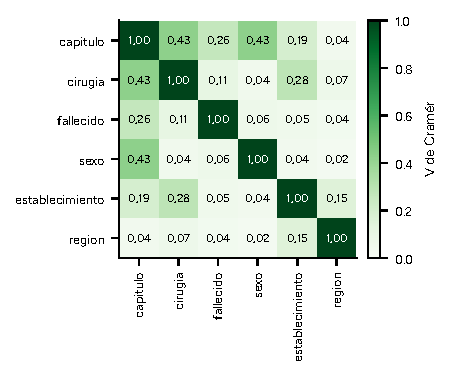
\includegraphics[width=0.85\linewidth]{figs/avance2_cramer.pdf}
\end{minipage}
\fuente
\end{figure}

\begin{figure}[H]
\centering
\caption{Histograma de la edad y gráficos Q-Q de los días, de $\ln$(días) y de la edad, en la muestra de 5.000 egresos de Shapiro--Wilk.}
\label{fig:anx-normal}
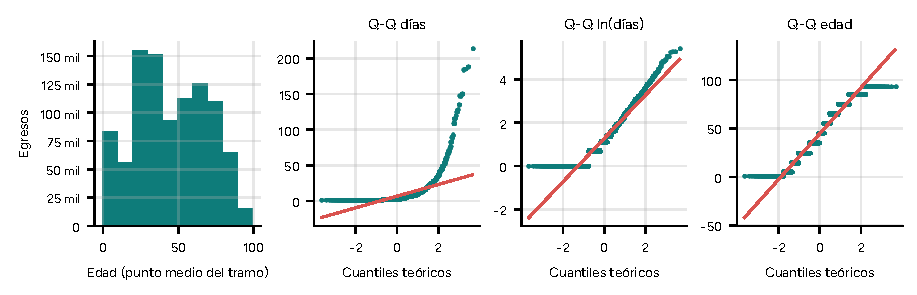
\includegraphics[width=\textwidth]{figs/anexo_normalidad.pdf}
\fuente
\end{figure}

\begin{figure}[H]
\centering
\caption{Distribución de $\ln$(días) por tramo de edad, región (ordenada por mediana), cirugía, condición de egreso, nacionalidad y pertenencia a pueblo originario. Sin puntos atípicos.}
\label{fig:anx-cajas}
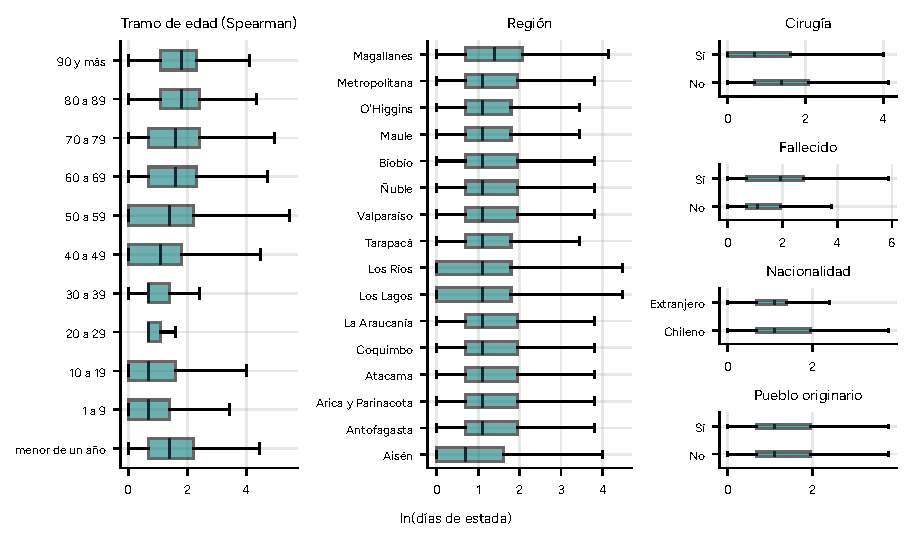
\includegraphics[width=\textwidth]{figs/anexo_cajas.pdf}
\fuente
\end{figure}

\begin{figure}[H]
\centering
\caption{Porcentaje de estadías prolongadas (más de 15 días) en cada categoría de los nueve factores del chi-cuadrado.}
\label{fig:anx-prol}
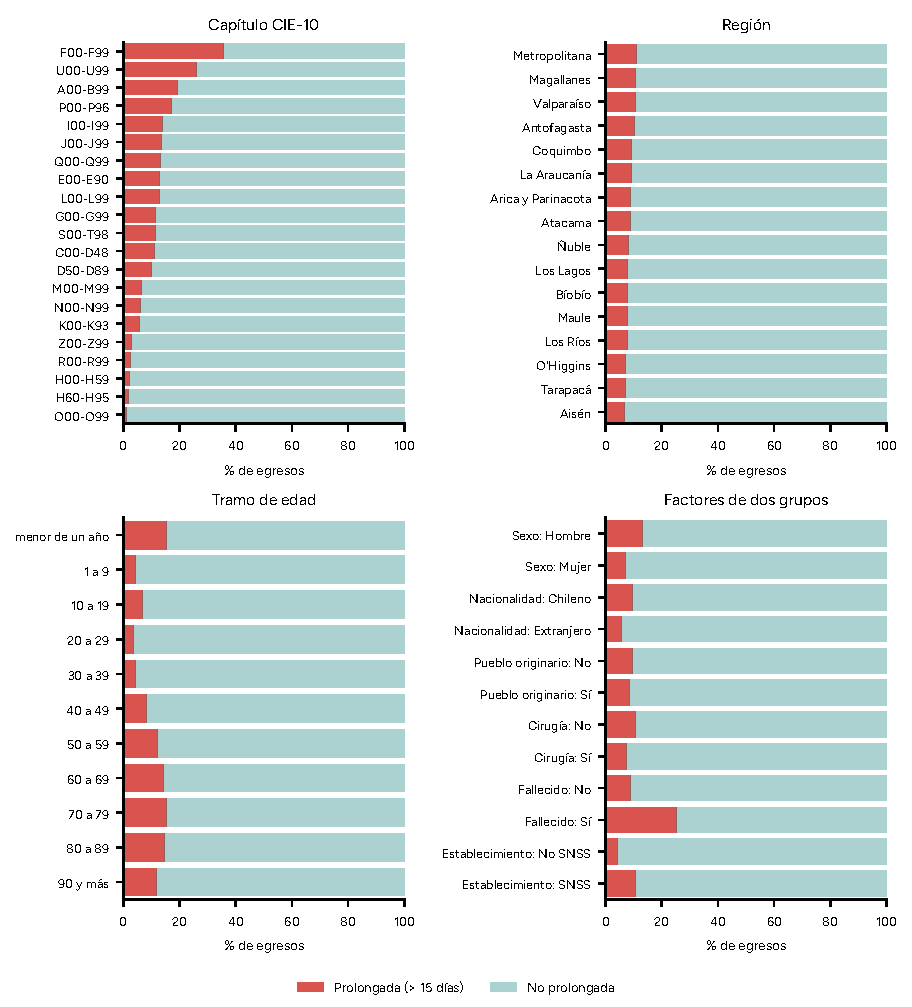
\includegraphics[width=\textwidth]{figs/anexo_prolongadas.pdf}
\fuente
\end{figure}

\clearpage
{\scriptsize\filas\renewcommand{\arraystretch}{1.0}
\setlength{\tabcolsep}{4pt}
\begin{longtable}{llrrrr}
\caption{Tablas de contingencia de cada factor con la estadía prolongada: egresos por categoría y porcentaje de prolongadas.}\label{tab:anx-cont}\\
\toprule
Factor & Categoría & No prolongada & Prolongada & Total & \% prolongadas \\
\midrule
\endfirsthead
\toprule
Factor & Categoría & No prolongada & Prolongada & Total & \% prolongadas \\
\midrule
\endhead
\bottomrule
\endfoot
\bottomrule
\multicolumn{6}{@{}l}{\cellcolor{white}\color{gris}Fuente: DEIS, MINSAL, egresos hospitalarios 2020; elaboración propia.}\\
\endlastfoot
\inputtab anexos/contingencia.tex
\end{longtable}}

% ---------------------------------------------------------------------
\clearpage
\section{Coeficientes completos de M3}\label{anx:coef}

Los 42 coeficientes de la regresión lineal de $\ln$(días). Las referencias son capítulo K00--K93, mujer, fuera del SNSS, sin cirugía, vivo y Región Metropolitana; la edad está centrada en 45,01 años. El valor-$p$ usa el error HC3 y $\%\Delta=100\,(e^{\beta}-1)$, con el intervalo del 95\pct{} clásico. En la edad, $\%\Delta$ es el cambio por año a la edad media; el término cuadrático no se lee por separado.

\begin{table}[H]
\centering\scriptsize\filas\renewcommand{\arraystretch}{1.08}
\caption{Coeficientes de M3 con error estándar clásico y HC3.}
\label{tab:anx-coef}
\setlength{\tabcolsep}{3.5pt}
\begin{tabular}{lrrrrrrr}
\toprule
Coeficiente & $\hat\beta$ & EE & EE HC3 & $t$ & Valor-$p$ & $\%\Delta$ & IC 95\pct{} de $\%\Delta$ \\
\midrule
\inputtab anexos/coef_m3.tex
\bottomrule
\end{tabular}
\fuente
\end{table}

\begin{figure}[H]
\centering
\caption{Cambio porcentual en la media geométrica ajustada de días asociado a cada coeficiente de M3, con intervalo de confianza del 95\pct{}.}
\label{fig:forest}
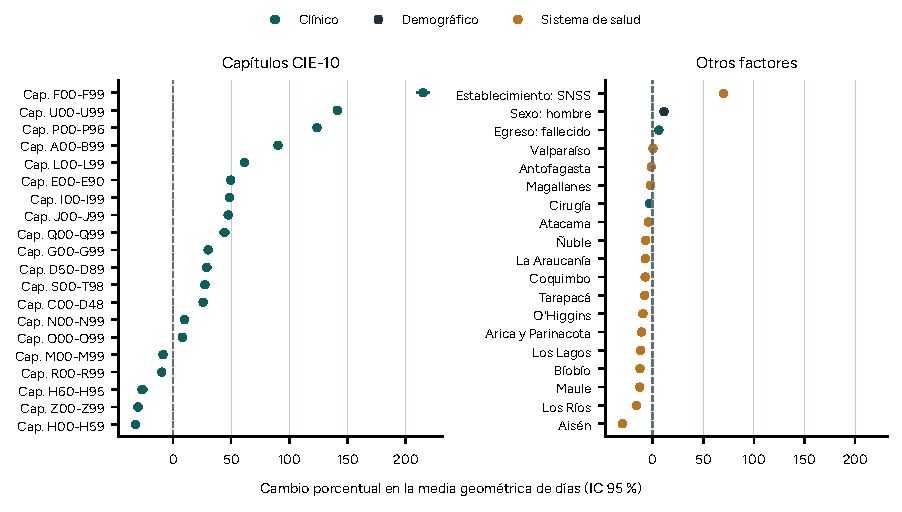
\includegraphics[width=\textwidth]{figs/forest.pdf}
\fuente
\end{figure}

% ---------------------------------------------------------------------
\clearpage
\section{Supuestos del modelo lineal}\label{anx:supuestos}

La figura~\ref{fig:resid} muestra los residuos de M3. La dispersión crece con el valor ajustado y el gráfico Q-Q se aparta de la recta en las colas. La figura~\ref{fig:edad} y las tablas~\ref{tab:anx-deciles} y \ref{tab:anx-edad} comparan lo ajustado con lo observado.

\begin{figure}[H]
\centering
\caption{Residuos frente a valores ajustados (con la media por ventiles), histograma de los residuos y gráfico Q-Q. Se grafica un subconjunto de puntos; las estadísticas usan todos los egresos.}
\label{fig:resid}
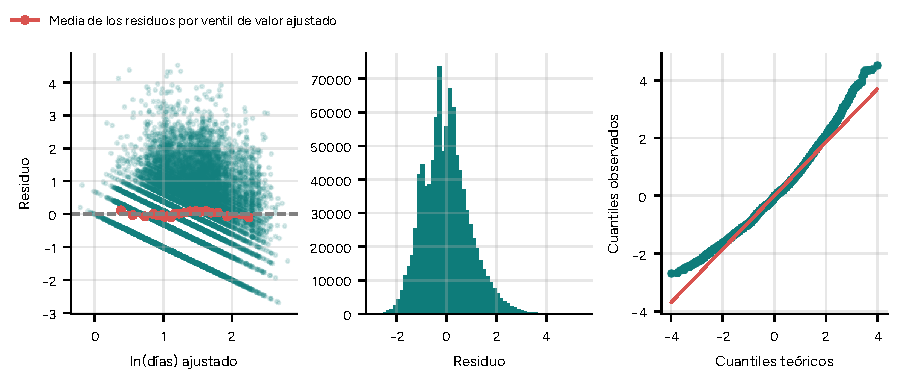
\includegraphics[width=\textwidth]{figs/avance2_residuos.pdf}
\fuente
\end{figure}

\begin{figure}[H]
\centering
\caption{Media observada de $\ln$(días) por tramo de edad y media ajustada por M3.}
\label{fig:edad}
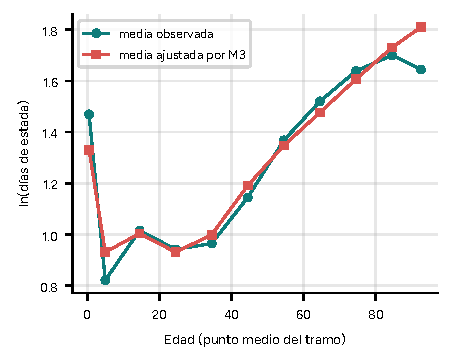
\includegraphics[width=0.5\textwidth]{figs/avance2_edad.pdf}
\fuente
\end{figure}

\begin{table}[H]
\centering\footnotesize\filas
\caption{Media geométrica ajustada y observada por decil de valor ajustado de M3.}
\label{tab:anx-deciles}
\begin{tabular}{rrrrr}
\toprule
Decil & Egresos & Ajustada (días) & Observada (días) & Mediana observada \\
\midrule
\inputtab anexos/deciles.tex
\bottomrule
\end{tabular}
\fuente
\end{table}

\begin{table}[H]
\centering\footnotesize\filas
\caption{Media de $\ln$(días) observada y ajustada por M3 en cada tramo de edad, y su media geométrica en días.}
\label{tab:anx-edad}
\begin{tabular}{lrrrrr}
\toprule
Tramo & Edad usada & $\ln$ observado & $\ln$ ajustado & Días observados & Días ajustados \\
\midrule
\inputtab anexos/edad.tex
\bottomrule
\end{tabular}
\fuente
\end{table}

% ---------------------------------------------------------------------
\clearpage
\section{Especificaciones alternativas y selección forward}\label{anx:sens}

La tabla~\ref{tab:sens} compara M3 con las especificaciones alternativas. Cada $F$ parcial de M4 a M6 contrasta el modelo con el anterior de la lista, y la última fila se compara con M3. La tabla~\ref{tab:anx-forward} muestra la selección forward por BIC sobre factores completos: en cada paso entra el factor que más baja el BIC y el recorrido se detiene cuando ninguno lo baja.

\begin{table}[H]
\centering\small\filas
\caption{Especificaciones M3 a M6 en la base completa.}
\label{tab:sens}
\begin{tabular}{lrrrrr}
\toprule
Modelo & $k$ & $R^2$ aj. & $\Delta$BIC & $F$ parcial (gl) & $\eta^2$ parcial \\
\midrule
M3 & 42 & 0,198 & --- & --- & --- \\
M4 (tramos de edad) & 50 & 0,202 & $-4.588$ & 589 (8) & 0,0048 \\
M5 (+ capítulo $\times$ establ.) & 70 & 0,214 & $-14.538$ & 746 (20) & 0,0152 \\
M6 (+ edad $\times$ establ.) & 80 & 0,215 & $-663$ & 80 (10) & 0,0008 \\
M3 + nacionalidad y etnia & 44 & 0,198 & $+12{,}6$ & 7,49 (2) & 0,00002 \\
\bottomrule
\end{tabular}
\fuente
\end{table}

\begin{table}[H]
\centering\small\filas
\caption{Selección forward por BIC de los factores del modelo lineal. Todas las $F$ parciales tienen $p<0{,}001$.}
\label{tab:anx-forward}
\begin{tabular}{rlrrrrr}
\toprule
Paso & Entra & $k$ & BIC & $\Delta$BIC & $R^2$ aj. & $F$ parcial \\
\midrule
\inputtab anexos/forward.tex
\bottomrule
\end{tabular}
\fuente
\end{table}

El recorrido llega al mismo M3 (BIC 2.601.099). La edad entra con sus dos términos para respetar la forma de M3.
\end{document}
